% Draft for submission to Nonlinearity (IOP Publishing / London Mathematical Society).
% IOP journals accept any reasonable LaTeX format at first submission; the IOP class (iopart or iopjournal)
% can be swapped in at acceptance. Compile with:  latexmk -pdf main.tex
\documentclass[11pt,a4paper]{article}

\usepackage[utf8]{inputenc}

\usepackage{amsmath,amssymb,amsthm,mathtools}
\usepackage{graphicx,booktabs,array}
\usepackage[margin=2.5cm]{geometry}
\usepackage{microtype}
\usepackage{xcolor}
\usepackage{enumitem}
\usepackage[colorlinks=true,linkcolor=blue!45!black,citecolor=blue!45!black,urlcolor=blue!45!black]{hyperref}
\usepackage[capitalise,nameinlink]{cleveref}

\newtheorem{theorem}{Theorem}[section]
\newtheorem{proposition}[theorem]{Proposition}
\newtheorem{lemma}[theorem]{Lemma}
\newtheorem{corollary}[theorem]{Corollary}
\newtheorem{conjecture}[theorem]{Conjecture}
\theoremstyle{definition}
\newtheorem{definition}[theorem]{Definition}
\newtheorem{example}[theorem]{Example}
\theoremstyle{remark}
\newtheorem{remark}[theorem]{Remark}
\crefname{conjecture}{Conjecture}{Conjectures}

\newcommand{\R}{\mathbb{R}}
\newcommand{\C}{\mathbb{C}}
\newcommand{\Id}{\mathrm{Id}}
\newcommand{\T}{\mathcal{T}}
\newcommand{\bI}{\mathbf{I}}
\newcommand{\bM}{\mathbf{M}}
\newcommand{\dd}{\mathrm{d}}
\newcommand{\Jq}{\mathbb{J}}
\newcommand{\tr}{^{\!\top}}
\DeclareMathOperator{\spn}{span}
\DeclareMathOperator{\rank}{rank}

\title{Kahan's method on quadratic lifts:\\[2pt]
modified invariants, Liouville measures and\\ integrable maps in every dimension}
% TODO(authors): complete the author list and affiliations before submission.
\author{Ben K.~Tapley\\[2pt]
\small SINTEF, Oslo, Norway\\
\small\texttt{ben.tapley@sintef.no}}
\date{Draft of \today}

\begin{document}
\maketitle

\begin{abstract}
Kahan's method discretises a quadratic vector field by a birational map that costs one linear solve per
step and that, remarkably often, inherits invariant measures, modified integrals and even integrability.
Quadratic lifts, i.e.\ auxiliary variables such as $y=x_ix_j$ or $u=\mathrm e^{q}$ that turn a polynomial or
exponential vector field into a quadratic one, carry the method far beyond quadratic problems, but the lift
constraints and the original invariants need not survive the discretisation. We determine which structures
do survive. (i)~A \emph{block theorem}: a block of variables that moves along fixed affine flows at affine
speeds keeps explicitly modified versions of all quadratic invariants of those flows, even when the flows do
not commute. It contains the two-variable theorem of Celledoni, McLaren, Owren and Quispel, produces modified
invariants with squared denominators for resonant blocks, and yields $I-\tfrac{h^2}{8}F\tr\nabla^2I\,F$ for
every quadratic integral whose curvature lies in affinely moving variables. (ii)~Lift constraints whose
factors move affinely are always protected, and the lifted method restricted to the invariant \emph{shifted
sheet} is a symmetric one-step method on the original variables. (iii)~For every potential built from
exponentials and single harmonics, with any mass matrix and in any dimension, the lifted Kahan map preserves
the canonical Liouville measure and a modified energy. (iv)~For isotropic quartic oscillators in $\R^n$ the
lifted Kahan map is integrable for every $n$: we give its modified energy, angular momenta and invariant
measure in closed form, show that regular level sets are invariant 2-tori carrying skew rotations, and obtain
an integrator of $O(n)$ cost per step that remains stable far beyond the St\"ormer--Verlet limit. Exact
degree-growth computations indicate that integrability survives lifting when it stems from linear symmetries
and one degree of freedom, and is lost when it rests on hidden symmetries.
\end{abstract}

\noindent\textbf{Keywords:} Kahan's method, Hirota--Kimura discretisation, quadratic lifts, auxiliary
variables, discrete integrable systems, invariant measures, geometric numerical integration.

\noindent\textbf{MSC 2020:} 37J70, 39A36, 65P10, 65L05.

% ======================================================================================================
\section{Introduction}\label{sec:intro}

Let $\dot z=F(z)$ be a quadratic vector field on $\R^N$, $F(z)=Q(z,z)+Bz+b$ with $Q$ symmetric and bilinear.
Kahan's method~\cite{Kahan93,KahanLi97} replaces it by the map $z\mapsto z'$ defined by
\begin{equation}\label{eq:kahan}
\frac{z'-z}{h}=Q(z,z')+\tfrac12B(z+z')+b .
\end{equation}
The new point enters linearly, so a step costs one linear solve. The method is symmetric and, when applied
to quadratic Hamiltonian systems with constant Poisson structure, it preserves a modified energy and an
invariant measure~\cite{CMOQ13}. Applied to integrable systems it produces integrable maps far more often
than one has a right to expect: the Euler and Lagrange tops~\cite{HirotaKimura00,KimuraHirota00}, the
Clebsch and Kirchhoff systems and many others~\cite{PPS09,PPS11,CMMOQ14,PetreraZander17,PSS19}, planar cubic
Hamiltonian systems~\cite{PSS19,GMQ24}, and cases where integrability can be restored by small adjustments of
the coefficients~\cite{PSZ20}. Kahan's method is therefore one of the few places where geometric numerical
integration~\cite{HLW06} and the theory of discrete integrable systems~\cite{Veselov91,Suris03} meet.

The method is defined only for quadratic vector fields. Polarisation extends it to higher degree at the price
of multistep schemes~\cite{CMMOQ15}, and Hone and Quispel construct explicit analogues for certain higher
order equations~\cite{HoneQuispel19}. Another route is a \emph{quadratic lift}. Introduce auxiliary variables,
for instance $y_{ij}=x_ix_j$, $u=\mathrm e^{\alpha\cdot q}$ or $(c,s)=(\cos\theta,\sin\theta)$, so that the
original system becomes the restriction of a quadratic system in more variables to an invariant ``sheet''.
Every polynomial vector field admits such a lift~\cite{Kerner81}, and lifts are widely used in model
reduction~\cite{Gu11,KramerWillcox19,BychkovPogudin21}. In geometric integration, auxiliary variables make
energy-stable schemes linear (the IEQ and SAV approaches~\cite{Yang16,ShenXuYang18}), and multiple quadratic
auxiliary variables allow the midpoint rule to preserve several invariants at once~\cite{Tapley22}.
Combining a quadratic lift with Kahan's method gives a linearly implicit one-step integrator for any
polynomial ODE, and for many non-polynomial ones.

The price is that Kahan's map lives in the lifted space. It need not preserve the sheet, and the integrals
and measures of the original system need not survive. This paper asks which structures do survive, and
whether lifting can produce new integrable maps. Our main results are the following.

\begin{enumerate}[leftmargin=*,label=(\roman*)]
\item \textbf{A block theorem} (\cref{thm:block}). If a block of variables moves as
  $\dot w=\sum_kA_k(z)L_k(w)$, with affine \emph{speeds} $A_k$ and fixed affine vector fields $L_k$, then
  Kahan's map conserves explicitly modified versions of all quadratic invariants of the $L_k$, provided the
  second-derivative operators of the $L_k$ close on these invariants and commute. The fields $L_k$
  themselves need not commute. The theorem contains the two-variable theorem of~\cite{CMOQ19}, gives
  modified invariants with squared denominators for resonant blocks (\cref{ex:resonant}), and yields
  $I_h=I-\tfrac{h^2}{8}F\tr\nabla^2I\,F$ whenever the curvature of a quadratic integral $I$ lies in variables
  that move affinely (\cref{cor:affine}).
\item \textbf{Lift constraints and the shifted sheet} (\cref{sec:lifts}). We classify the lift constraints
  $y-x_ix_j$ that are exact integrals (\cref{prop:classify}). Those whose factors move affinely are always
  protected, as $y-x_ix_j+\tfrac{h^2}{4}\dot x_i\dot x_j$ (\cref{thm:affine-constraints}). On the invariant
  ``shifted sheet'' that these modified constraints define, the lifted method is a symmetric second-order
  one-step method on the original variables (\cref{thm:sheet}).
\item \textbf{Liouville measures} (\cref{thm:liouville}). For every Hamiltonian
  $\frac12p\tr Gp+\sum_kc_k\mathrm e^{\alpha_k\cdot q}+\sum_jg_j\cos(\beta_j\cdot q)$, in any dimension and with
  any constant mass matrix, Kahan's method in the exponential and harmonic variables preserves the
  canonical Liouville measure and a modified energy. This covers Toda chains, rotor and XY chains and coupled
  pendula.
\item \textbf{An integrable family in every dimension} (\cref{thm:isotropic,cor:tori}). For
  $H=\frac12\lvert p\rvert^2+U(\lvert q\rvert^2)$ with $U$ quadratic and $q,p\in\R^n$, the lift
  $y=\lvert q\rvert^2$ gives a Kahan map that conserves modified angular momenta, a modified energy and an
  explicit measure, for every $n$. Its regular level sets are invariant 2-tori on which it acts as a skew
  rotation. The map can be evaluated in closed form at $O(n)$ cost (\cref{rem:explicit}), and it remains
  stable far beyond the St\"ormer--Verlet limit (\cref{sec:numerics}).
\item \textbf{Which integrable systems survive lifting} (\cref{sec:survey}). Exact degree-growth computations
  on nineteen lifted maps indicate that the lifted Kahan map is integrable when the original integrability
  comes from linear symmetries plus one degree of freedom, and is not when it rests on hidden symmetries
  (\cref{conj:principle}).
\end{enumerate}

\paragraph{Relation to other work.}
A companion manuscript~\cite{LP} studies Kahan's method for Lie--Poisson systems through a Cayley form of the
map. Its ``midpoint theorem'' covers the single-speed case of our block theorem and the commuting cases of
our measure results. Our block theorem does not need commuting coefficient matrices, which is what the
isotropic family requires (\cref{rem:LP}). Conversely, \cite{LP} proves, with computer assistance, that every three-dimensional
quadratic Nambu system has a Kahan-invariant measure, which we use in \cref{sec:onedof}. Integrable Kahan maps
in arbitrary dimension are known for Lotka--Volterra systems~\cite{KQV16,vdKMMQ24} and for almost abelian
Lie--Poisson systems~\cite{LP}; the family of \cref{sec:isotropic} is of a different kind, coming from a
mechanical system with a non-quadratic potential through a lift. Integrable discretisations of central-force
and quartic-potential problems have been constructed by other
means~\cite{MinesakiNakamura02,FengMaruno08,Suris03}, and discrete-gradient methods preserve energy and
angular momentum~\cite{MQR99}. What is new in \cref{sec:isotropic} is that integrability arises from a
general-purpose, linearly implicit integrator, with all modified integrals and the measure in closed form and
in every dimension.

\paragraph{Outline.}
\Cref{sec:prelim} collects facts about Kahan's method and defines quadratic lifts. \Cref{sec:block} proves the
block theorem and its corollaries. \Cref{sec:lifts} treats lift constraints and the shifted sheet,
\cref{sec:measures} invariant measures, and \cref{sec:isotropic} the isotropic family. \Cref{sec:survey}
surveys integrability, \cref{sec:numerics} gives numerical experiments, and \cref{sec:conclusion} lists open
problems. \Cref{app:proof} describes an independent computer-algebra verification of \cref{thm:isotropic},
and \cref{app:exact} the exact searches.

% ======================================================================================================
\section{Preliminaries}\label{sec:prelim}

\subsection{Kahan's method}

Throughout, $F(z)=Q(z,z)+Bz+b$ is a quadratic vector field on $\R^N$, $F'(z)=2Q(z,\cdot)+B$ is its Jacobian
matrix, and $\Phi_h\colon z\mapsto z'$ is Kahan's map~\eqref{eq:kahan}. We collect standard facts, see
\cite{CMOQ13,CMMOQ14}.

\begin{proposition}\label{prop:basic}
\begin{enumerate}[label=(\alph*)]
\item $\Phi_h(z)=z+h\big(\Id-\tfrac h2F'(z)\big)^{-1}F(z)$; $\Phi_h$ is birational and $\Phi_h^{-1}=\Phi_{-h}$.
\item If $a,b$ are affine functions, Kahan's method discretises the quadratic term $a(z)b(z)$ as
  $\tfrac12[a(z)b(z')+a(z')b(z)]$.
\item Kahan's method commutes with affine changes of variables: if $z=Tw+c$ with $T$ invertible and
  $G(w)=T^{-1}F(Tw+c)$, then the Kahan map of $G$ is $w\mapsto T^{-1}(\Phi_h(Tw+c)-c)$.
\item $\det D\Phi_h(z)=\det\big(\Id+\tfrac h2F'(z')\big)/\det\big(\Id-\tfrac h2F'(z)\big)$.
\item Every linear first integral of $F$ is a first integral of $\Phi_h$.
\end{enumerate}
\end{proposition}

\begin{definition}
Let $I$ be a function on $\R^N$. A \emph{modified integral} of $I$ is a function $I_h$, rational in $z$ and
smooth in $h$ near $h=0$, with $I_0=I$ and $I_h\circ\Phi_h=I_h$. We call $I$ \emph{protected} if it has a
modified integral. A measure $\mu=\dd z/P(z)$ with $P$ rational is \emph{preserved} if
\begin{equation}\label{eq:measure}
P(\Phi_h(z))=\det D\Phi_h(z)\,P(z),
\end{equation}
i.e.\ $P$ is a discrete Darboux function whose cofactor is the Jacobian determinant~\cite{CEMOQTvdK19}.
\end{definition}

\begin{lemma}\label{lem:protected}
A protected function is a first integral of $F$, and the protected functions form a vector space.
\end{lemma}

\begin{proof}
$0=I_h(\Phi_h(z))-I_h(z)=h\,\nabla I(z)\cdot F(z)+O(h^2)$. The second claim holds because modified integrals
can be added.
\end{proof}

\subsection{Quadratic lifts}

\begin{definition}\label{def:lift}
Let $\dot x=f(x)$ be an ODE on $\R^n$. A \emph{quadratic lift} consists of a map $\psi\colon\R^n\to\R^m$ and a
quadratic vector field $F$ on $\R^{n+m}$ with $F(x,\psi(x))=\big(f(x),D\psi(x)f(x)\big)$. The \emph{sheet}
$\Sigma=\{y=\psi(x)\}$ is invariant under the flow of $F$, and the flow on $\Sigma$ projects to the flow of $f$.
The components of $c=y-\psi(x)$ are the \emph{constraints}. A constraint is \emph{exact} if it is a first
integral of $F$ on all of $\R^{n+m}$, and \emph{conditional} if its derivative vanishes only on $\Sigma$. The
\emph{lifted Kahan method} is Kahan's method applied to $F$.
\end{definition}

The lift is not unique: on $\Sigma$, a cubic term $q^3$ may be written $qy$, $yq$ or a combination with other
monomials. By \cref{lem:protected}, conditional constraints are never protected.

\begin{example}[the quartic oscillator]\label{ex:quartic}
For $H=\frac12p^2+\frac14q^4$ and $y=q^2$, the lifted field is $\dot q=p$, $\dot p=-qy$, $\dot y=2qp$. The
constraint $c=y-q^2$ is exact, and so is the lifted energy $\tilde H=\frac12p^2+\frac14y^2$. Kahan's map
conserves $c_h=y-q^2+\tfrac{h^2}{4}p^2$ and $\tilde H_h=\tilde H/(1+\frac12h^2q^2)$, and it preserves
$\dd q\,\dd p\,\dd y/(1+\frac12h^2q^2)$. Both integrals follow from \cref{sec:block}.
\end{example}

% ======================================================================================================
\section{The block theorem}\label{sec:block}

\subsection{Statement and proof}

Let $P\colon\R^N\to\R^m$ be linear and $w=Pz$ a block of linear coordinates. Suppose that
\begin{equation}\label{eq:blockfield}
PF(z)=\sum_{k=1}^rA_k(z)\,L_k(Pz),
\end{equation}
where the \emph{speeds} $A_k\colon\R^N\to\R$ are affine and the $L_k(w)=L_kw+\ell_k$ are fixed affine vector
fields on $\R^m$. For a function $I$ of degree at most two on $\R^m$, with Hessian $\nabla^2I$, define
\[
(\T_{kl}I)(w)=L_k(w)\tr\,\nabla^2I\,L_l(w).
\]

\begin{lemma}[crossed identity]\label{lem:crossed}
Assume~\eqref{eq:blockfield}, let $z'=\Phi_h(z)$, $w=Pz$, $w'=Pz'$, $a_k=\frac h2A_k(z)$ and
$a_k'=\frac h2A_k(z')$. Then
\begin{equation}\label{eq:blockstep}
w'-\sum_ka_kL_k(w')=w+\sum_ka_k'L_k(w),
\end{equation}
and every polynomial $I$ of degree at most two on $\R^m$ that is a first integral of every $L_k$ satisfies
\begin{equation}\label{eq:crossedgen}
I(w')+\frac12\sum_{k,l}a_ka_l\,(\T_{kl}I)(w')=I(w)+\frac12\sum_{k,l}a_k'a_l'\,(\T_{kl}I)(w).
\end{equation}
\end{lemma}

\begin{proof}
By \cref{prop:basic}(b), applied to each product in~\eqref{eq:blockfield}, the $w$-components of Kahan's
equations read $w'-w=\frac h2\sum_k\big[A_k(z)L_k(w')+A_k(z')L_k(w)\big]$, which is~\eqref{eq:blockstep}.
Since $I$ is quadratic, Taylor's formula is exact, and since $\nabla I\cdot L_k=0$,
$I\big(w\pm\sum_ka_kL_k(w)\big)=I(w)+\frac12\sum_{k,l}a_ka_l(\T_{kl}I)(w)$. Applying $I$ to both sides
of~\eqref{eq:blockstep} gives~\eqref{eq:crossedgen}.
\end{proof}

\begin{theorem}[block theorem]\label{thm:block}
Let $V$ be a finite-dimensional space of polynomials of degree at most two on $\R^m$, each a first integral
of every $L_k$, and assume that $\T_{kl}V\subset V$ for all $k,l$. Choose a basis $\bI=(I_1,\dots,I_d)$ of $V$
and let $T_{kl}$ be the matrices with $\T_{kl}I_i=\sum_j(T_{kl})_{ij}I_j$. If the matrices $T_{kl}$ commute
pairwise, then the vector of functions
\begin{equation}\label{eq:blockinv}
\bI_h(z)=\bM_h(z)^{-1}\,\bI(Pz),\qquad\bM_h(z)=\Id+\frac{h^2}{8}\sum_{k,l=1}^rA_k(z)A_l(z)\,T_{kl},
\end{equation}
is conserved by Kahan's map wherever $\bM_h$ is invertible.
\end{theorem}

\begin{proof}
Apply \cref{lem:crossed} to each basis element. With $\bM(a)=\Id+\frac12\sum_{k,l}a_ka_lT_{kl}$ we obtain
$\bM(a)\bI(w')=\bM(a')\bI(w)$. The matrices $\bM(a)$ and $\bM(a')$ are polynomials in the commuting $T_{kl}$,
so they commute, and therefore $\bM(a')^{-1}\bI(w')=\bM(a)^{-1}\bI(w)$. Since $\bM(a)=\bM_h(z)$ and
$\bM(a')=\bM_h(z')$, this is the claim.
\end{proof}

The ``speeds'' cross over in~\eqref{eq:blockstep}: the speed at the old point multiplies the new point and
vice versa. If all $a_k=a_k'$, \eqref{eq:blockstep} is a Cayley transform and conserves every element of $V$
exactly. The rescaling $\bM_h$ is the exact price of sampling the speeds at different ends of the step.

\subsection{Consequences}

\begin{corollary}[two variables, \cite{CMOQ19}]\label{cor:twovar}
Let $w=Pz\in\R^2$ and $I(w)=\frac12a_1w_1^2+a_2w_1w_2+\frac12a_3w_2^2+a_4w_1+a_5w_2$. If
$\dot w=A(z)J\nabla I(w)$ with $A$ affine and $J=\left(\begin{smallmatrix}0&1\\-1&0\end{smallmatrix}\right)$,
then Kahan's map conserves
\[
I_h=\frac{I+\frac18h^2D_2A^2}{1+\frac14h^2D_1A^2},\qquad D_1=a_1a_3-a_2^2,\quad D_2=2a_2a_4a_5-a_3a_4^2-a_1a_5^2.
\]
\end{corollary}

\begin{proof}
Take $V=\spn\{I,1\}$ and $L(w)=J\nabla I(w)$. With $S=\nabla^2I$ and $s=(a_4,a_5)\tr$ we have
$J\tr SJ=\operatorname{adj}S$, hence
$\T I=(Sw+s)\tr\operatorname{adj}(S)(Sw+s)=2D_1I-D_2$ and $\T1=0$. Inverting the $2\times2$ triangular matrix
$\bM_h$ gives the formula.
\end{proof}

\begin{corollary}[affine factors]\label{cor:affine}
Let $I(z)=\frac12z\tr Sz+s\tr z$ be a first integral of $F$ with $S\,Q(u,v)=0$ for all $u,v$, i.e.\ every
linear form in the range of $S$ has an affine time derivative. Then
\[
I_h=I-\frac{h^2}{8}F(z)\tr S\,F(z)
\]
is a modified integral.
\end{corollary}

\begin{proof}
Write $S=R\tr\Lambda R$ with $R$ of full row rank and $\Lambda$ symmetric and invertible, and let $\phi=Rz$
and $\eta=s\tr z$. Since $RQ=0$, $\dot\phi=\alpha(z)$ with $\alpha$ affine, and $\nabla I\cdot F=0$ gives
$\dot\eta=-\phi\tr\Lambda\alpha(z)$. The block $w=(\phi,\eta)$ therefore moves as
$\dot w=\sum_j\alpha_j(z)L_j(w)$ with $L_j(w)=(e_j,-(\Lambda\phi)_j)$. The function
$\tilde I(w)=\frac12\phi\tr\Lambda\phi+\eta$ equals $I$, is invariant under every $L_j$, and satisfies
$\T_{jk}\tilde I=\Lambda_{jk}$ and $\T_{jk}1=0$. All $T_{jk}$ are multiples of one nilpotent matrix, so
\cref{thm:block} applies and gives $I_h=I-\frac{h^2}8\alpha\tr\Lambda\alpha=I-\frac{h^2}8F\tr SF$.
\end{proof}

\begin{example}\label{ex:ishii}
For $\dot x=y$, $\dot y=z$, $\dot z=12xy$ the integral $I=z-6x^2$ has $S=-12e_xe_x\tr$, and $\dot x$ is
linear. \Cref{cor:affine} gives $I_h=z-6x^2+\frac32h^2y^2$, an invariant found by direct computation
in~\cite{CMMOQ14}. In \cref{ex:quartic}, the corollary gives $c_h$.
\end{example}

\begin{example}[resonant blocks]\label{ex:resonant}
Let $\Jq$ be a $2\times2$ rotation by a right angle and let a block $(u,v)\in\R^2\times\R^2$ move as
$\dot u=A(z)(\omega\Jq u+v)$, $\dot v=A(z)\,\omega\Jq v$. The quadratic invariants of the fixed (Jordan-block)
flow include $N=\lvert v\rvert^2$ and $G=u\tr\Jq v$, and $\T N=2\omega^2N$, $\T G=2\omega^2G-2\omega N$. With
$\beta=\frac14h^2\omega^2A(z)^2$, \cref{thm:block} gives
\[
N_h=\frac{N}{1+\beta},\qquad G_h=\frac{G}{1+\beta}+\frac{\beta N/\omega}{(1+\beta)^2}.
\]
The squared denominator is not produced by \cref{cor:twovar,cor:affine}: in normal-mode coordinates $G$ is not
a sum of two-variable integrals, and its Hessian does not annihilate the quadratic part.
\end{example}

\begin{example}[non-commuting fields: isotropic angular momenta]\label{ex:angmom}
For $H=\frac12\lvert p\rvert^2+U(\lvert q\rvert^2)$ with $U$ quadratic, lifted by $y=\lvert q\rvert^2$, the
block $w=(q,p)\in\R^{2n}$ moves as $\dot w=1\cdot L_1(w)+2U'(y)\cdot L_2(w)$ with $L_1(q,p)=(p,0)$ and
$L_2(q,p)=(0,-q)$. These shear fields do not commute; together with $[L_1,L_2]$ they span
$\mathfrak{sl}(2)$. The angular momenta $M_{ab}=q_ap_b-q_bp_a$ are invariant under both, and
$\T_{11}M_{ab}=\T_{22}M_{ab}=0$, $\T_{12}M_{ab}=\T_{21}M_{ab}=M_{ab}$. \Cref{thm:block} gives the modified
angular momenta
\[
M_{ab,h}=\frac{M_{ab}}{1+\frac12h^2U'(y)} .
\]
\end{example}

\begin{remark}\label{rem:LP}
When all coefficient matrices of the Cayley form of Kahan's map commute, \cite{LP} shows that $z$ and $z'$
share a ``midpoint'' at which every compatible quadratic form is conserved. This covers
\cref{cor:twovar}, \cref{cor:affine} and the single-speed case of \cref{thm:block}. In
\cref{ex:angmom} the coefficient matrices do not commute: their commutator is a non-zero diagonal matrix.
\Cref{thm:block} only needs the operators $\T_{kl}$ to commute \emph{on $V$}. For the generalised Suslov
systems $\dot x=\ell(x)J_0\mathsf Hx$ of~\cite{CMMOQ14}, \cref{thm:block} gives one modified integral
$I_k/(1+\frac14h^2\ell(x)^2\omega_k^2)$ for each normal-mode action $I_k$ with frequency $\omega_k$.
\end{remark}

% ======================================================================================================
\section{Lift constraints and the shifted sheet}\label{sec:lifts}

\subsection{Which constraints are exact, and which are protected}

\begin{proposition}\label{prop:classify}
Let $c=y-x_ix_j$ be a first integral of a quadratic field $F$, where $y,x_i,x_j$ are coordinates, and write
$F_i=Q_i+(\text{affine})$, $F_j=Q_j+(\text{affine})$ with quadratic forms $Q_i,Q_j$. Then
$x_jQ_i+x_iQ_j=0$. Consequently:
\begin{enumerate}[label=(\alph*)]
\item if $i=j$, then $Q_i=0$;
\item if $i\ne j$, then either $Q_i=Q_j=0$, or $Q_i=x_iR$ and $Q_j=-x_jR$ for a non-zero linear form $R$.
\end{enumerate}
\end{proposition}

\begin{proof}
$\nabla c\cdot F=F_y-x_jF_i-x_iF_j=0$, and $F_y$ is quadratic, so the cubic part $x_jQ_i+x_iQ_j$ vanishes.
For $i=j$ this gives $Q_i=0$. For $i\ne j$ the coordinates $x_i$ and $x_j$ are coprime, so $x_i$ divides
$Q_i$; writing $Q_i=x_iR$ gives $Q_j=-x_jR$.
\end{proof}

In case (b) with $R\ne0$ the two factors are stretched and squeezed at the same rate, like
$(q,p)\mapsto(\mathrm e^\tau q,\mathrm e^{-\tau}p)$. We call this \emph{opposite scaling}.

\begin{theorem}\label{thm:affine-constraints}
If $c=y-x_ix_j$ is a first integral and $\dot x_i=F_i$, $\dot x_j=F_j$ are affine (cases (a) and (b) with
$Q_i=Q_j=0$), then
\[
c_h=y-x_ix_j+\frac{h^2}{4}F_i(z)F_j(z)
\]
is a modified integral.
\end{theorem}

\begin{proof}
Apply \cref{cor:affine}: $S=-(e_ie_j\tr+e_je_i\tr)$ annihilates $Q$ exactly when $Q_i=Q_j=0$, and
$F\tr SF=-2F_iF_j$.
\end{proof}

\begin{corollary}[mechanical systems with quartic potentials]\label{cor:mech}
Let $H=\frac12p\tr Gp+V(q)$ with $G$ constant and $V$ a polynomial of degree at most four, and lift with
$Y=(y_{ij})=qq\tr$. For every lifted field with $\dot q=Gp$ and $\dot Y=\dot qq\tr+q\dot q\tr$, Kahan's map
conserves the matrix $Y-qq\tr+\frac{h^2}{4}(Gp)(Gp)\tr$.
\end{corollary}

In case (b) with $R\ne0$, \cref{thm:block} does not apply. The block $(x_i,x_j,y)$ moves along the scaling
field $(x_i,-x_j,0)$ and the translation fields $(1,0,x_j)$, $(0,1,x_i)$, and the second derivative of $c$
along the scaling field, $2x_ix_j$, is not an invariant of the translations, so closure fails. Such a
constraint can still be protected through a \emph{partner}, i.e.\ by lying in the vector space of
\cref{lem:protected}. \Cref{prop:pencil} gives an example.

\subsection{Back-substitution: the shifted sheet}

\begin{theorem}\label{thm:sheet}
Let $F$ be a quadratic lift of $\dot x=f(x)$ whose constraints $c=y-\psi(x)$ all have modified integrals of
the form $c_h=c+h^2r_h(x,y)$ with $r_h$ smooth. For $h$ small, the \emph{shifted sheet}
$\Sigma_h=\{c_h=0\}$ is locally the graph of $y=\psi_h(x)=\psi(x)+O(h^2)$, it is invariant under $\Phi_h$,
and the induced map $\varphi_h\colon x\mapsto x'$ is a one-step method of order two for $\dot x=f(x)$. If
$c_{-h}=c_h$, then $\varphi_h$ is symmetric, $\varphi_h^{-1}=\varphi_{-h}$. One step costs one linear solve
of size $n+m$.
\end{theorem}

\begin{proof}
The implicit function theorem gives $\psi_h$, since $\partial c_h/\partial y=\Id+O(h^2)$. Invariance follows
from $c_h\circ\Phi_h=c_h$. Since $\Phi_h(z)=z+O(h)$ and $\Phi_h(z+\delta)=\Phi_h(z)+\delta+O(h\delta)$,
starting at $(x,\psi_h(x))$ instead of $(x,\psi(x))$ changes the $x$-component of the step by $O(h^3)$. On
$\Sigma$ the exact flow of $F$ projects to that of $f$, and Kahan's method has order two, so $\varphi_h$ has
order two. If $c_{-h}=c_h$ then $\Sigma_{-h}=\Sigma_h$, and $\Phi_h^{-1}=\Phi_{-h}$ gives
$\varphi_h^{-1}=\varphi_{-h}$.
\end{proof}

\begin{example}\label{ex:backsub}
For the quartic oscillator, $\Sigma_h=\{y=q^2-\frac{h^2}4p^2\}$ and substituting into Kahan's equations gives
\[
q'=q+\tfrac h2(p+p'),\qquad p'=p-\tfrac h2\,qq'(q+q')+\tfrac{h^3}{8}\big(qp'^2+q'p^2\big).
\]
This symmetric map of the plane is \emph{nonlinearly} implicit in $(q,p)$, yet the lifted form computes it
with one linear solve. For mechanical lifts (\cref{cor:mech}) the shifted sheet is explicit,
$Y=qq\tr-\frac{h^2}{4}(Gp)(Gp)\tr$.
\end{example}

\subsection{One degree of freedom: protection through a partner}

Let $x=(q,p)\in\R^2$ and consider $H=U(\varphi(x))+\kappa(x)$ with $\varphi=\frac12x\tr\Phi x$,
$\kappa=\frac12x\tr Kx$ and $U(y)=\frac12u_2y^2+u_1y$, $u_2\ne0$. Lift with $y=\varphi(x)$ and
$\tilde H=U(y)+\kappa(x)$. The lifted field is the Nambu field $\dot z=\nabla\tilde H\times\nabla c$ on
$z=(q,p,y)$, with $c=y-\varphi(x)$. This covers all even quartic oscillators ($\varphi=q^2$) and, for
$\varphi=qp$, an opposite-scaling constraint.

\begin{proposition}[essentially {\cite[Theorem~2]{CMOQ19}}]\label{prop:pencil}
Let $\lambda_1\ne\lambda_2$ be the roots of $\det(K-\lambda\Phi)=0$ (real, or complex conjugate; one may lie
at infinity when $\det\Phi=0$). Then each pencil member $I_\lambda=\tilde H+\lambda c$ is a two-variable
integral, $K-\lambda\Phi=\mu_\lambda\ell_\lambda\ell_\lambda\tr$, and with $A_\lambda=\ell_\lambda\tr J\Phi x$,
\[
I_{\lambda,h}=\frac{I_\lambda-\frac18h^2\mu_\lambda(u_1+\lambda)^2A_\lambda^2}{1+\frac14h^2\mu_\lambda u_2A_\lambda^2}.
\]
Hence $c_h=(I_{\lambda_1,h}-I_{\lambda_2,h})/(\lambda_1-\lambda_2)$ and $\tilde H_h$ are conserved, the measure
$\dd z/(D_{\lambda_1}D_{\lambda_2})$ with $D_\lambda=1+\frac14h^2\mu_\lambda u_2A_\lambda^2$ is preserved, and
the lifted Kahan map is integrable.
\end{proposition}

\begin{proof}[Proof sketch]
In the coordinates $(\ell_{\lambda_1}\tr x,y,\ell_{\lambda_2}\tr x)$ both pencil members are two-variable
functions sharing $y$, and $\nabla\tilde H\times\nabla c$ is a constant multiple of
$\nabla I_{\lambda_1}\times\nabla I_{\lambda_2}$. This is the integrable class of \cite[Theorem~2]{CMOQ19};
the formula for $I_{\lambda,h}$ is \cref{cor:twovar}.
\end{proof}

\begin{remark}[limits of protection]\label{rem:limits}
Protection reaches one level deep: by \cref{cor:affine}, the \emph{factors} of a constraint must move
affinely. In mechanical systems these are the positions, so lifts by products of positions are protected;
they represent potentials of degree at most four. A sextic potential needs products of lifted variables,
whose velocities are quadratic, and the corresponding constraints are conditional. Rewriting a product by
polarisation, $x_ix_j=\frac12[(x_i+x_j)^2-x_i^2-x_j^2]$, does not help: the condition $SQ=0$ is invariant
under linear changes of variables (\cref{prop:basic}(c)). Exponentials and single harmonics escape the
one-level rule, because their derivatives stay in the span of the lifted variables (\cref{sec:measures}).
\end{remark}

% ======================================================================================================
\section{Invariant measures}\label{sec:measures}

\subsection{Exponential and trigonometric potentials: the Liouville measure}

Consider, on $\R^n\times\R^n$,
\begin{equation}\label{eq:exptrig}
H=\tfrac12p\tr Gp+\sum_{k=1}^Kc_k\,\mathrm e^{\alpha_k\cdot q}+\sum_{j=1}^Jg_j\cos(\beta_j\cdot q),
\end{equation}
with a constant matrix $G$ and arbitrary vectors $\alpha_k,\beta_j\in\R^n$ (dependent or not). With
$u_k=\mathrm e^{\alpha_k\cdot q}$ and $(C_j,S_j)=(\cos\beta_j\cdot q,\sin\beta_j\cdot q)$, drop $q$ and consider
the quadratic system
\begin{equation}\label{eq:exptriglift}
\dot p=-\sum_kc_ku_k\alpha_k+\sum_jg_jS_j\beta_j,\quad
\dot u_k=(\alpha_k\tr Gp)\,u_k,\quad
\dot C_j=-(\beta_j\tr Gp)\,S_j,\quad \dot S_j=(\beta_j\tr Gp)\,C_j .
\end{equation}

\begin{theorem}\label{thm:liouville}
Kahan's map of~\eqref{eq:exptriglift} preserves the measure
\[
\dd p\ \prod_{k=1}^K\frac{\dd u_k}{\lvert u_k\rvert}\ \prod_{j=1}^J\frac{\dd C_j\,\dd S_j}{C_j^2+S_j^2}
\]
for any matrix $G$. If $G$ is symmetric it also conserves
$E_h=\frac12p\tr Gp+\sum_kc_ku_k+\sum_jg_jC_j-\frac{h^2}{8}\dot p\tr G\dot p$, with $\dot p$ given by
\eqref{eq:exptriglift}, and each modified circle $(C_j^2+S_j^2)/(1+\frac14h^2(\beta_j\tr Gp)^2)$.
\end{theorem}

\begin{proof}
Write $a_k=\alpha_k\tr Gp$, $b_j=\beta_j\tr Gp$, $\zeta_j=C_j+\mathrm iS_j$, and primes for the new values. By
\cref{prop:basic}(b) Kahan's equations are
\[
u_k'\big(1-\tfrac h2a_k\big)=u_k\big(1+\tfrac h2a_k'\big),\qquad
\zeta_j'\big(1-\tfrac{\mathrm ih}2b_j\big)=\zeta_j\big(1+\tfrac{\mathrm ih}2b_j'\big),
\]
and $p'-p=\frac h2\big[-\sum_kc_k\alpha_k(u_k+u_k')+\sum_jg_j\beta_j(S_j+S_j')\big]$. Define intermediate
variables $\hat u_k=u_k/(1-\frac h2a_k)$ and $\hat\zeta_j=\zeta_j/(1-\frac{\mathrm ih}2b_j)$. Then
$u_k+u_k'=\hat u_k(2+\frac h2\alpha_k\tr G\delta)$ and
$S_j+S_j'=2\hat S_j+\frac h2\hat C_j\beta_j\tr G\delta$, where $\delta=p'-p$, so the momentum equation becomes
\[
\Big(\Id+\frac{h^2}{4}\Big[\sum_kc_k\hat u_k\alpha_k\alpha_k\tr-\sum_jg_j\hat C_j\beta_j\beta_j\tr\Big]G\Big)\delta
=-h\sum_kc_k\hat u_k\alpha_k+h\sum_jg_j\hat S_j\beta_j .
\]
Thus $\delta$ depends only on $(\hat u,\hat\zeta)$. In the coordinates $p$, $x_k=\log\lvert u_k\rvert$,
$\rho_j=\log\lvert\zeta_j\rvert$, $\theta_j=\arg\zeta_j$, one step is the composition of three shears:
$(x,\rho,\theta)$ is shifted by a function of $p$; then $p$ is shifted by $\delta(\hat u,\hat\zeta)$; then
$(x,\rho,\theta)$ is shifted by a function of $p'$. Each shear preserves $\dd p\,\dd x\,\dd\rho\,\dd\theta$,
which is the stated measure. The energy is \cref{cor:affine}: $\dot p$ is linear in $(u,S)$, so the Hessian of
the lifted energy, which is $G$ on the $p$-block, annihilates $Q$. Taking moduli in the $\zeta_j$-equation gives
the circles.
\end{proof}

\begin{corollary}\label{cor:toda}
For the open and periodic Toda chains, rotor and XY chains with nearest-neighbour coupling, and coupled
pendula with a non-diagonal mass matrix, the lifted Kahan method is a reversible, volume-preserving,
linearly implicit one-step method that conserves a modified energy (and, for Toda, the total momentum).
\end{corollary}

The map is not symplectic: numerically, the Kahan--Toda map violates the Poisson property by $O(1)$ amounts.
Volume preservation by Runge--Kutta methods, of which Kahan's method on quadratic fields is an
instance~\cite{CMMOQ14}, is studied in~\cite{BMQW16}.
The Liouville measure is $h$-independent, which is unusual for Kahan maps, whose densities typically depend on
$h$. Volume preservation and reversibility are the two properties required of an integrator in Hybrid Monte
Carlo~\cite{DKPR87}, so \cref{thm:liouville} provides linearly implicit candidates for that purpose.

\subsection{One degree of freedom: an area form on the shifted sheet}\label{sec:onedof}

Every lift of a one-degree-of-freedom potential of degree at most four with $y=q^2$ is a Nambu field
$\nabla\tilde H\times\nabla c$ on $\R^3$ with quadratic $\tilde H$ and $c=y-q^2$: write $V$ as a quadratic
$\tilde V(q,y)$; then $\dot q=p$, $\dot p=-\tilde V_q-2q\tilde V_y$, $\dot y=2qp$. Kahan maps of three-dimensional quadratic systems have a rich structure~\cite{HonePetrera09,CMMOQ14,PS18}.
The companion manuscript~\cite{LP} proves, with computer assistance, that Kahan's map of every
three-dimensional Nambu field with quadratic $H$ and $C$ preserves a measure $\dd z/P$ with $P$ a polynomial of
degree at most four. Our
exact searches (\cref{app:exact}) independently found such densities for four quartic potentials and for
random quadratic Nambu systems, including a closed form valid for all $h$ for
$V=\frac14q^4+\frac13q^3+\frac12q^2$.

\begin{corollary}\label{cor:area}
Assume the result of~\cite{LP} quoted above. For every quartic potential, the back-substituted method of
\cref{thm:sheet} preserves the area form $\dd q\wedge\dd p/P(q,p,q^2-\frac{h^2}4p^2)$.
\end{corollary}

\begin{proof}
On the invariant level set $\{c_h=0\}$ the preserved measure $\dd z/P$ induces the invariant form $\omega$
with $\dd z/P=\dd c_h\wedge\omega$. Since $\partial c_h/\partial y=1$, its pull-back along the graph
$y=q^2-\frac{h^2}4p^2$ is $\dd q\wedge\dd p/P$.
\end{proof}

For a non-symmetric quartic such as $V=\frac14q^4+\frac13q^3+\frac12q^2$, no modified energy is conserved and
the degree growth is exponential (\cref{sec:survey}). The back-substituted map is then an area-preserving
near-identity map that is not integrable. Area preservation is what KAM-type arguments such as Moser's twist
theorem~\cite{Moser62} require in order to produce invariant curves that confine orbits, and it is consistent
with the bounded energy error observed in practice.

\subsection{Measures are rare beyond these classes}

Exact searches for polynomial densities (\cref{app:exact}) find none for the lifted Kahan maps of two-site
$\varphi^4$ and Fermi--Pasta--Ulam lattices (degree at most six) and of the two-site discrete nonlinear
Schr\"odinger equation (degree at most four). This agrees with the conjecture of~\cite{LP} that, for generic
quadratic Hamiltonians, Kahan's map of a Lie--Poisson system keeps a measure only for linear systems (two-step
nilpotent algebras) and in one degree of freedom; the lifted lattices are affine Lie--Poisson systems on
nilpotent algebras of higher step. Beyond three dimensions, measure preservation is a structural property: it comes
from symmetry (\cref{sec:isotropic}) or from exponential and harmonic variables (\cref{thm:liouville}).

% ======================================================================================================
\section{An integrable family in every dimension}\label{sec:isotropic}

Let $n\ge2$, $U(y)=\frac12u_2y^2+u_1y$ with $u_2\ne0$, and
$H=\frac12\lvert p\rvert^2+U(\lvert q\rvert^2)$ on $\R^n\times\R^n$, a particle in a rotation-invariant
anharmonic well. The lift $y=\lvert q\rvert^2$ gives the quadratic field on $\R^{2n+1}$
\begin{equation}\label{eq:isofield}
\dot q=p,\qquad\dot p=-2U'(y)\,q,\qquad\dot y=2\,q\cdot p .
\end{equation}
Write $Y(z)=1+\frac12h^2U'(y)$, $M_{ab}=q_ap_b-q_bp_a$, and
$K(z)=\frac12\lvert p\rvert^2+U(y)+\frac{u_1^2}{2u_2}=\frac12\lvert p\rvert^2+\frac{u_2}2\big(y+\frac{u_1}{u_2}\big)^2$.

\begin{theorem}\label{thm:isotropic}
Kahan's map $\Phi_h$ of~\eqref{eq:isofield} has the following properties.
\begin{enumerate}[label=(\alph*)]
\item It is $O(n)$-equivariant and $(q',p')$ lies in $\spn\{q,p\}$: explicitly
  $\binom{q'}{p'}=N\binom{q}{p}$ for a $2\times2$ matrix $N=N(z,z')$ acting on the pair, with
  $\det N=Y(z')/Y(z)$. In particular $q\wedge q'=h\,q\wedge p/Y(z)$.
\item It conserves
\begin{gather*}
c_h=y-\lvert q\rvert^2+\frac{h^2}{4}\lvert p\rvert^2,\qquad
M_{ab,h}=\frac{M_{ab}}{Y},\\
E_h=\frac{K+\frac12h^2u_2\lvert M_h\rvert^2}{D},\qquad D=1+h^2u_2\lvert q\rvert^2-\frac12h^4u_2K,
\end{gather*}
  where $\lvert M_h\rvert^2=\sum_{a<b}M_{ab,h}^2$.
\item It preserves the measure $\dd z/P_n$ with $P_n=Y^{\,n-1}D$. More precisely,
  $\det D\Phi_h(z)=\big(Y(z')/Y(z)\big)^{n-1}D(z')/D(z)$.
\end{enumerate}
\end{theorem}

The linear term $u_1$ enters only through $\tilde y=y+u_1/u_2$: in the variables $(q,p,\tilde y)$ the field
\eqref{eq:isofield} reads $\dot q=p$, $\dot p=-2u_2\tilde yq$, $\dot{\tilde y}=2q\cdot p$, and
$Y=1+\frac12h^2u_2\tilde y$, $K=\frac12\lvert p\rvert^2+\frac12u_2\tilde y^2$. Since Kahan's method commutes with
this affine change of variables, the case $u_1\ne0$ is the case $u_1=0$ on another level set of $c_h$. We
write $\kappa=h^2u_2$ and use primes for values at $z'$.

\begin{proof}
(a) By \cref{prop:basic}(b) Kahan's equations are
\begin{equation}\label{eq:isokahan}
q'-q=\tfrac h2(p+p'),\qquad p'-p=-\alpha q'-\alpha'q,\qquad y'-y=h(q\cdot p'+q'\cdot p),
\end{equation}
where $\alpha=hU'(y)$ and $\alpha'=hU'(y')$. The first two say
$\left(\begin{smallmatrix}1&-h/2\\ \alpha&1\end{smallmatrix}\right)\binom{q'}{p'}
=\left(\begin{smallmatrix}1&h/2\\-\alpha'&1\end{smallmatrix}\right)\binom qp$, where each entry multiplies
vectors in $\R^n$. Hence
$N=\frac1Y\left(\begin{smallmatrix}1-h\alpha'/2&h\\-\alpha-\alpha'&1-h\alpha/2\end{smallmatrix}\right)$ and
$\det N=(1+\frac h2\alpha')/(1+\frac h2\alpha)=Y'/Y$. Equivariance holds because~\eqref{eq:isofield} is
$O(n)$-equivariant (\cref{prop:basic}(c)).

(b) $c_h$ is \cref{thm:affine-constraints}. Since $q'\wedge p'=\det N\,q\wedge p$, we get
$M'_{ab}/Y'=M_{ab}/Y$; this is also \cref{ex:angmom}.

For $E_h$, consider the block $w=(p,\tilde y)$. It moves as $\dot w=\sum_kq_k\,L_k(w)$, with the coordinates $q_k$
as speeds and the fixed linear fields $L_k(w)=(-2u_2\tilde y\,e_k,\ 2p_k)$, and $K(w)$ is invariant under every
$L_k$. The closure condition of \cref{thm:block} fails, but \cref{lem:crossed} still applies. With
$a=\frac h2q$ and $a'=\frac h2q'$ it gives
$K(w')+\frac12\sum_{k,l}a_ka_l(\T_{kl}K)(w')=K(w)+\frac12\sum_{k,l}a_k'a_l'(\T_{kl}K)(w)$, and here
$\sum_{k,l}x_kx_l(\T_{kl}K)(w)=4u_2\big(u_2\tilde y^2\lvert x\rvert^2+(x\cdot p)^2\big)
=4u_2\big(2K\lvert x\rvert^2-\lvert x\wedge p\rvert^2\big)$ by Lagrange's identity. Hence
\begin{equation}\label{eq:crossed}
K'\big(1+\kappa\lvert q\rvert^2\big)-\tfrac12\kappa\lvert q\wedge p'\rvert^2
=K\big(1+\kappa\lvert q'\rvert^2\big)-\tfrac12\kappa\lvert q'\wedge p\rvert^2 .
\end{equation}
By (a) and the first equation in~\eqref{eq:isokahan}, $q\wedge p'=\frac2h\,q\wedge q'-q\wedge p=(2-Y)M_h$ and
$q'\wedge p=\frac2h\,q\wedge q'-q'\wedge p'=(2-Y')M_h$. Conservation of $c_h$ gives
$\lvert q\rvert^2=\tilde y+\frac{h^2}2K-\frac{h^2}4u_2\tilde y^2-g$ and the same expression with primes, with the
same constant $g$. Substitute these into~\eqref{eq:crossed}; the terms in $KK'$ cancel. With
$\lambda=\frac12\kappa\lvert M_h\rvert^2$, $s=2-Y=1-\frac12\kappa\tilde y$ and $\mu=2-\kappa g$, what remains is
$K'(\mu-s^2)-\lambda s^2=K(\mu-s'^2)-\lambda s'^2$, that is,
\[
(K'+\lambda)(\mu-s^2)=(K+\lambda)(\mu-s'^2).
\]
Finally $\mu-s^2=1+\kappa\tilde y-\frac14\kappa^2\tilde y^2-\kappa g=D$ and $\mu-s'^2=D'$, so $E_h'=E_h$.

(c) Put $v=q-\frac h2p$, $w=q+\frac h2p$ and $w'=q'+\frac h2p'$. The first equation in~\eqref{eq:isokahan} says
$w=q'-\frac h2p'$, so $q=\frac12(v+w)$ and $q'=\frac12(w+w')$. Let $A=v\cdot w$, $B=w\cdot w'$ and
$C=\lvert w\rvert^2$. In these variables the third equation in~\eqref{eq:isokahan} reads $y'-y=B-A$, and the
second one reads $Yw'+Y'v=(4-Y-Y')\,w$. Hence
\begin{equation}\label{eq:R12}
Y'-Y=\tfrac12\kappa(B-A),\qquad YB+Y'A=(4-Y-Y')\,C .
\end{equation}
Moreover $D=(2-Y)Y+\kappa A$ and $D'=(2-Y')Y'+\kappa B$, because $1-\frac14\kappa^2\tilde y^2=(2-Y)Y$ and
$\lvert q\rvert^2-\frac{h^2}4\lvert p\rvert^2=v\cdot w$. A Schur-complement computation in the block form of
$\Id\mp\frac h2F'$ gives
\begin{align*}
\det\big(\Id-\tfrac h2F'(z)\big)&=Y^{n-1}\big(Y+\kappa\,q\cdot w\big)=Y^{n-1}\big(Y+\tfrac12\kappa(A+C)\big),\\
\det\big(\Id+\tfrac h2F'(z')\big)&=Y'^{\,n-1}\big(Y'+\kappa\,q'\cdot w\big)=Y'^{\,n-1}\big(Y'+\tfrac12\kappa(B+C)\big).
\end{align*}
Using~\eqref{eq:R12}, a short computation shows
\[
2D=(4-Y-Y')\big(Y+\tfrac12\kappa(A+C)\big),\qquad 2D'=(4-Y-Y')\big(Y'+\tfrac12\kappa(B+C)\big).
\]
For the first identity, expand the right-hand side, replace $(4-Y-Y')C$ by $YB+Y'A$, and then
$\frac12\kappa(B-A)$ by $Y'-Y$; the second follows by symmetry. Dividing the two identities and using
\cref{prop:basic}(d) gives $\det D\Phi_h=(Y'/Y)^{n-1}D'/D$, which is equivalent to $P_n(z')=\det D\Phi_h\,P_n(z)$.
\end{proof}

The integrals and the measure were first found by exact searches for Darboux polynomials (\cref{app:exact}).
The proofs explain their form. The angular momenta come from the block theorem with non-commuting fields. The
energy comes from a block $(p,\tilde y)$ that fails the closure condition only by the term
$\lvert q\wedge p\rvert^2$, which the conserved discrete angular momentum absorbs. The measure density is
$Y^{n-1}$ times the denominator of $E_h$. For $M=0$, $E_h$ is a function of the two-variable integral
$K/(1+\kappa\lvert q\rvert^2)$ of \cref{cor:twovar}. In the notes accompanying this paper the energy appears in the
equivalent form $E_h/(1+\frac12h^4u_2E_h)$. All identities were also verified independently by computer algebra
(\cref{app:proof}).

\begin{corollary}[integrability]\label{cor:tori}
For $n=2$ the integrals $c_h$, $M_h$, $E_h$ are functionally independent. Let $L$ be a compact connected
component of a regular level set with $M_h\ne0$ on which $\Phi_h^{\pm1}$ are defined and $P_2\ne0$, and assume
$\Phi_h(L)=L$ and that the induced circle map below preserves orientation (both hold for small $h$). Then $L$
is a 2-torus and $\Phi_h|_L$ is smoothly conjugate to a skew rotation
\[
(\theta,\phi)\mapsto(\theta+\rho,\ \phi+g(\theta)),\qquad(\theta,\phi)\in\mathbb T^2 .
\]
If $\rho$ is Diophantine, $\Phi_h|_L$ is conjugate to a translation of $\mathbb T^2$, i.e.\ the motion is
quasi-periodic. For $n>2$ the same holds on the level sets of $c_h$, $E_h$ and all $M_{ab,h}$, which comprise
$2n-1$ independent integrals on $\R^{2n+1}$.
\end{corollary}

\begin{proof}
A $3\times3$ minor of the Jacobian of $(c_h,M_h,E_h)$ is a non-zero rational function (\cref{app:proof}), which
gives functional independence. $L$ is a compact, orientable 2-manifold, being a regular level set in $\R^5$.
Rotations of the pair $(q,p)$ preserve the integrals, so the connected group $SO(2)$ maps $L$ to itself; it acts
freely because $M\ne0$. A compact orientable surface with a free circle action is a torus, and $L/SO(2)$ is a
circle. $\Phi_h$ commutes with the action, so it induces a homeomorphism $f$ of $L/SO(2)$. The measure
$\dd z/P_2$ induces on $L$ the invariant density $\sigma=(\dd z/P_2)/(\dd c_h\wedge\dd M_h\wedge\dd E_h)$, which
is smooth, nowhere zero and rotation invariant, so $\lvert\sigma\rvert$ descends to a smooth positive
$f$-invariant density on the circle. Its distribution function conjugates $f$ to a rigid rotation by $\rho$. Choosing a section of the
trivial principal bundle $L\to L/SO(2)$ gives coordinates $(\theta,\phi)$ in which $SO(2)$ acts by translating
$\phi$; since $\Phi_h$ commutes with these translations, it has the stated form. For Diophantine $\rho$ the
cohomological equation $\gamma(\theta+\rho)-\gamma(\theta)=g(\theta)-\bar g$ has a smooth solution, and
$\phi\mapsto\phi-\gamma(\theta)$ conjugates to the translation by $(\rho,\bar g)$. For $n>2$, fixing all
$M_{ab,h}$ fixes the oriented plane $\Pi$ (the bivector $M_h$ is decomposable, giving $2n-3$ independent
components) and reduces to $n=2$.
\end{proof}

\begin{proposition}[bounded orbits]\label{prop:bounded}
Let $u_2>0$. If $D(z_0)>0$, for instance if $h^4u_2K(z_0)<2$, then the orbit of $z_0$ under $\Phi_h$ is bounded,
as long as it is defined.
\end{proposition}

\begin{proof}
Let $e=E_h(z_0)\ge0$ and $c=c_h(z_0)$. Along the orbit $K+\frac12\kappa\lvert M_h\rvert^2=eD$, hence
$K\big(1+\frac12eh^4u_2\big)\le e\big(1+\kappa\lvert q\rvert^2\big)$, that is,
$K\le e_*\big(1+\kappa\lvert q\rvert^2\big)$ with $e_*=e/(1+\frac12eh^4u_2)$ and $e_*h^4u_2<2$. Put
$s=\frac{h^2}{4}\lvert p\rvert^2\ge0$ and $t=\lvert q\rvert^2-s$, so that $y=c+t$. The inequality becomes
\[
s\Big(\frac{2}{h^2}-e_*h^2u_2\Big)+\frac{u_2}{2}\Big(t+c+\frac{u_1}{u_2}\Big)^2-e_*h^2u_2\,t\le e_* .
\]
The coefficient of $s$ is positive, so the inequality bounds $t$ (a quadratic with positive leading coefficient)
and then $s$. Hence $\lvert q\rvert^2=t+s$, $\lvert p\rvert^2$ and $y$ stay bounded.
\end{proof}

\begin{remark}[an $O(n)$ explicit form]\label{rem:explicit}
Eliminating $q',p'$ from Kahan's equations leaves one scalar linear equation for $y'$. With
$\alpha=hU'(y)$, $Y=1+\frac h2\alpha$ and $w=q+\frac h2p$,
\begin{gather*}
y'=\frac{yY+h\big(2p-(\alpha+hu_1)q\big)\cdot w}{Y+\kappa\,q\cdot w},\\
q'=\frac{(1-\frac h2\alpha')q+hp}{Y},\qquad
p'=\frac{(1-\frac h2\alpha)p-(\alpha+\alpha')q}{Y},
\end{gather*}
with $\alpha'=hU'(y')$. A step therefore costs $O(n)$ operations, like one St\"ormer--Verlet step, and no
linear system has to be solved. The denominators vanish exactly where
$\det(\Id-\frac h2F')=Y^{n-1}(Y+\kappa\,q\cdot w)$ does. Two further identities make the link with
discrete Newtonian equations~\cite{Suris03}. Along an orbit $(q_k,p_k,y_k)$,
\[
q_k\wedge q_{k+1}=h\,M_h,\qquad q_{k+1}+q_{k-1}=\lambda_k\,q_k,\quad
\lambda_k=\frac{2-\frac12h^2\big(U'(y_{k+1})+U'(y_{k-1})\big)}{1+\frac12h^2U'(y_k)} .
\]
The first identity exhibits $M_h$ as the discrete angular momentum, and the second is a ``central force''
recurrence in which the force is evaluated through the auxiliary sequence $y_k$. With the initial value
$y_0=\lvert q_0\rvert^2-\frac{h^2}4\lvert p_0\rvert^2$ on the shifted sheet, $(q_k,p_k)$ is a symmetric,
second-order, integrable discretisation of the original system on $\R^{2n}$ (\cref{thm:sheet}).
\end{remark}

% ======================================================================================================
\section{Which integrable systems survive lifting?}\label{sec:survey}

\Cref{prop:pencil,thm:isotropic} produce integrable maps from systems whose integrability has a simple
origin: one degree of freedom, possibly after reduction by a linear symmetry. To see how far this goes, we
computed the degree growth of iterates for nineteen lifted Kahan maps. Kahan maps are birational; restricted
to a generic line, the $k$-th iterate has some degree $d_k$, and zero algebraic entropy
$\lim_{k\to\infty}\frac1k\log d_k=0$, in practice polynomial growth of $d_k$, is the standard indicator of
integrability~\cite{HietarintaViallet98,BellonViallet99}. We computed $d_k$ exactly, modulo a large prime
(\cref{app:exact}). \Cref{tab:degrees} and \cref{fig:degrees} summarise the results.

\begin{table}[t]
\centering\small
\caption{Degree growth $d_1,d_2,\dots$ of lifted Kahan maps (exact, modulo a prime, along a random line).
Quadratic growth indicates integrability, exponential growth chaos. ``Source'' names the origin of the
continuous system's integrability. Lifts use $y=\lvert q\rvert^2$ for isotropic systems, $y_k=q_k^2$ (or the
products noted) for quartic potentials, and exponential or harmonic variables otherwise.}
\label{tab:degrees}
\begin{tabular}{@{}lll@{}}
\toprule
Lifted system & $d_1,d_2,\dots$ & Source of integrability\\
\midrule
\multicolumn{3}{@{}l}{\emph{Integrable lifted maps}}\\
quartic oscillator ($\R^3$) & $3,9,19,33,51,73,99$ & one degree of freedom\\
isotropic quartic, $n=2,3,4$ & $4,12,25,44,68,97,132$ & rotations, one d.o.f.\\
isotropic quartic plus harmonic term & $4,12,25,44,68,97$ & rotations, one d.o.f.\\
isotropic quartic, magnetic field ($n=2$) & $4,13,28,49,76,109$ & rotations, one d.o.f.\\
decoupled $q_1^4+q_2^4$ & $5,17,37,65,101,145$ & decoupling\\
$1{:}6{:}1$ quartic, lift in $q_1\pm q_2$ & $5,17,37,65,101,145$ & decoupling after rotation\\
two-particle Toda & $2,4,6,8,10,12$ & translation, one d.o.f.\\
two coupled rotors & $3,9,19,33,51,73$ & translation, one d.o.f.\\
\midrule
\multicolumn{3}{@{}l}{\emph{Non-integrable lifted maps}}\\
$1{:}6{:}1$ quartic, lift $y_k=q_k^2$ & $5,25,113,>400$ & same system, unadapted lift\\
quartic $1{:}6{:}8$ and $1{:}12{:}16$ & $5,25,113,>400$ & hidden quartic integral\\
Garnier, $a_1\ne a_2$ & $4,16,58,208,>400$ & separation in elliptic coordinates\\
open Toda, three particles & $3,9,23,57,139,337,815$ & Lax pair\\
anisotropic $(q_1^2+2q_2^2)^2$ & $4,16,58,208,742$ & none (not integrable)\\
sextic isotropic & $5,16,43,114,305,>400$ & rotations; lift not fully protected\\
non-symmetric quartic, one d.o.f. & $3,9,23,57,139,337,815$ & one d.o.f.; energy not protected\\
prolonged Euler top ($v=\dot x$) & $4,16,52,160,>400$ & integrals not protected\\
\bottomrule
\end{tabular}
\end{table}

\begin{figure}[t]
\centering
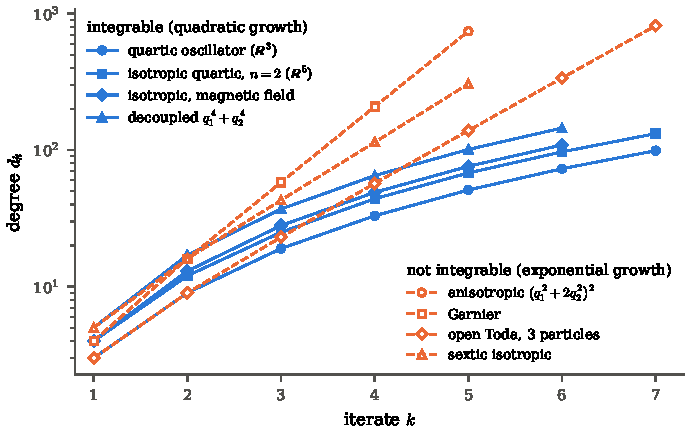
\includegraphics[width=0.72\textwidth]{fig_degrees.pdf}
\caption{Degree growth of representative lifted Kahan maps (logarithmic scale). Integrable maps (blue, solid)
grow quadratically; non-integrable ones (orange, dashed) grow exponentially. The Garnier sequence coincides
with the anisotropic one for $k\le4$.}
\label{fig:degrees}
\end{figure}

Three observations stand out. First, the isotropic family stays integrable with a harmonic term, in
dimensions three and four, and in a uniform magnetic field. Second, in our tests every lifted system whose
continuous integrability rests on a hidden symmetry is chaotic after lifting: three-particle Toda, the Garnier
system~\cite{Garnier19}, and the quartic potentials $1{:}6{:}8$ and $1{:}12{:}16$~\cite{Hietarinta87}. Third,
the separable $1{:}6{:}1$ potential $q_1^4+6q_1^2q_2^2+q_2^4=\frac12[(q_1+q_2)^4+(q_1-q_2)^4]$ gives an
integrable map with a lift in the separating coordinates $q_1\pm q_2$ and a chaotic map with the lift
$y_k=q_k^2$. Kahan's method commutes with linear changes of variables, but these two lifts are not related by
one, so the lift must respect the linear structure that makes the system integrable.

\begin{conjecture}\label{conj:principle}
Let $\dot x=f(x)$ be integrable because of a group of linear symmetries together with a reduction to one
degree of freedom, and let $F$ be a quadratic lift that is equivariant under the symmetries, adapted to the
reduction and has only protected constraints. If the reduced one-degree-of-freedom problem lies in a class
on which Kahan's method is integrable (\cref{prop:pencil}, or the single-exponential and single-harmonic
cases of \cref{thm:liouville}), then the lifted Kahan map is integrable.
\end{conjecture}

The heuristic reason is that every mechanism producing exact modified integrals here is linear-algebraic:
Kahan's method commutes with linear maps, and the modified integrals are built from quadratic invariants of
linear flows and their speeds. A linear symmetry therefore passes to the map, while hidden integrals (Toda's
$\operatorname{tr}L^3$, Garnier's Uhlenbeck integrals, the quartic integrals of $1{:}6{:}8$) are not invariants
of linear flows and nothing protects them. This is a statement about \emph{lifted} systems only: the
genuinely quadratic Clebsch and $\mathfrak{so}(4)$ Manakov tops keep hidden quadratic integrals under Kahan's
method~\cite{PPS09,PPS11}.

The magnetic case shows that \cref{thm:block} is sufficient but not necessary for protection. In velocity
variables, $\dot q=v$, $\dot v=-2U'(y)q+B\,\Jq v$, $\dot y=2q\cdot v$, the canonical angular momentum fails the
closure condition of \cref{thm:block}, yet the degree growth is quadratic. For $U(y)=\frac14y^2$, $B=1$ and
$h=\frac15$, an exact search finds two invariant densities $\dd z/P_1$ and $\dd z/P_2$ with polynomials $P_1$,
$P_2$ of degrees three and four. Their ratio is a rational integral, conserved to round-off, that mixes
$q\wedge v$ with energy-like terms. No mechanism in this paper predicts it.

% ======================================================================================================
\section{Numerical experiments}\label{sec:numerics}

We test the isotropic family as an integrator for a stiff anharmonic oscillator,
\[
H=\tfrac12\lvert p\rvert^2+\tfrac12\omega^2\lvert q\rvert^2+\tfrac14\lvert q\rvert^4,\qquad q,p\in\R^3,\quad
\omega=10,
\]
i.e.\ $u_2=\frac12$ and $u_1=\frac12\omega^2$, with $q_0=(0.8,0.1,-0.3)$, $p_0=(0,3,1)$ and $y_0$ on the
shifted sheet. The stiff harmonic term sits in the linear part of the lift, which Kahan's method treats like
the midpoint rule. We compare with the implicit midpoint rule on $(q,p)$, solved by Newton's method to a
tolerance of $10^{-14}$, and with the St\"ormer--Verlet method. \Cref{fig:isotropic} shows the results.

\begin{figure}[t]
\centering
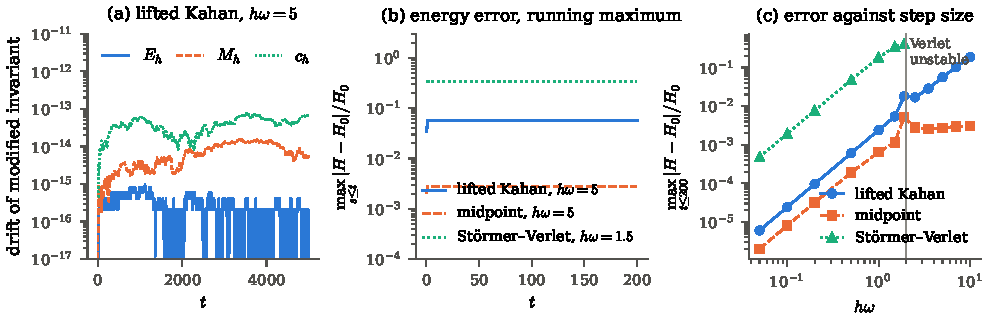
\includegraphics[width=\textwidth]{fig_isotropic.pdf}
\caption{Stiff isotropic oscillator in $\R^3$, $\omega=10$. (a) Lifted Kahan at $h\omega=5$: drift of the
modified invariants over $10^4$ steps (relative for $E_h$ and $M_h$, absolute for $c_h$). (b) Running maximum
of the relative energy error. (c) Maximal relative energy error on $[0,200]$ against $h\omega$;
St\"ormer--Verlet is unstable for $h\omega>2$.}
\label{fig:isotropic}
\end{figure}

\begin{itemize}[leftmargin=*]
\item \emph{Exact invariants.} At $h\omega=5$ the modified invariants $E_h$, $M_h$ and $c_h$ drift by at most
  $2\times10^{-16}$, $1.6\times10^{-14}$ and $7.7\times10^{-14}$ over $10^4$ steps, i.e.\ by round-off. The
  true energy error stays bounded at $5.6\times10^{-2}$.
\item \emph{Stability.} St\"ormer--Verlet is unstable for $h\omega>2$. The lifted Kahan map remained bounded
  for all tested step sizes up to $h\omega=10$. \Cref{prop:bounded} guarantees bounded orbits when
  $D(z_0)>0$. For this problem that holds for $h\omega$ below about $2$, because the constant
  $u_1^2/(2u_2)=\omega^4/4$ dominates $K$; the observed stability beyond that is not covered by the
  proposition.
\item \emph{Accuracy and cost.} At equal step size the energy error of the lifted Kahan map is about three times
  that of the midpoint rule for $h\omega\le1$, and it grows to $0.19$ at $h\omega=10$, where the midpoint
  error saturates at $3\times10^{-3}$. The midpoint rule needed three to four Newton iterations per step, each
  with a $6\times6$ linear solve, whereas the lifted Kahan step (\cref{rem:explicit}) costs about as much as a
  St\"ormer--Verlet step.
\end{itemize}

So the lifted Kahan map is an explicit-cost, symmetric, integrable integrator whose qualitative long-time
behaviour (invariant tori, exact modified energy and angular momenta) is correct at step sizes where the
standard explicit method fails. It is less accurate than the fully implicit midpoint rule at large
$h\omega$. For the exponential and trigonometric class of \cref{thm:liouville}, stiffness that enters through
the lifted nonlinear variables limits the step size: for a stiff rotor chain the lifted Kahan method conserved
its modified energy and stayed stable up to time $600$ for $h\omega\le2$, and blew up beyond.

% ======================================================================================================
\section{Conclusions and open problems}\label{sec:conclusion}

Quadratic lifts let Kahan's method act on polynomial, exponential and trigonometric problems. Exact modified
integrals survive through a few linear-algebraic mechanisms, collected in \cref{thm:block}: affinely moving
factors, two-variable integrals, and blocks that move along fixed linear flows at affine speeds, possibly
several and non-commuting. These mechanisms protect the lift constraints of quartic potentials, give the
Liouville measure for exponential and harmonic potentials, and make the lifted isotropic quartic oscillator
integrable in every dimension, with an $O(n)$ explicit form. Open problems:
\begin{enumerate}[leftmargin=*]
\item \emph{A block theorem without closure.} The proof of \cref{thm:isotropic}(b) uses a block whose
  closure defect is absorbed by another conserved quantity. A general version of this mechanism, or a reduction
  theory for Kahan maps with linear symmetries, might explain the magnetic case and prove
  \cref{conj:principle}.
\item \emph{The magnetic case.} Explain the rational integral of the magnetic isotropic map, and test
  dimensions $n\ge3$.
\item \emph{Explicit solutions.} The invariant tori of \cref{cor:tori} should admit a parametrisation by
  elliptic functions, as for planar Kahan maps~\cite{PSS19}.
\item \emph{Higher order.} Modified integrals depend on $h$, so compositions of Kahan steps with different
  step sizes conserve none of them exactly. Is there a lift or a composition that keeps a common invariant?
\item \emph{Applications.} Volume-preserving, reversible, linearly implicit integrators for exponential and
  rotor lattices (\cref{cor:toda}) are natural candidates for Hybrid Monte Carlo~\cite{DKPR87}; their
  acceptance rates remain to be tested.
\end{enumerate}

\section*{Acknowledgements}
% TODO(authors): funding and acknowledgements. Adapt the disclosure below to the journal's AI policy.
[To be completed.] Parts of the symbolic and numerical computations and of the drafting of this manuscript
were carried out with the assistance of an AI system; all results were checked by the author.

\section*{Data availability}
The scripts that reproduce every computation and figure, including the computer-algebra verification of
\cref{thm:isotropic}, are available at [repository URL to be added].

% ======================================================================================================
\appendix
\section{Computer-algebra verification of \texorpdfstring{\cref{thm:isotropic}}{Theorem 6.1}}
\label{app:proof}

The proofs of \cref{thm:isotropic} in \cref{sec:isotropic} are complete without computer assistance. As an
independent check, three SymPy~1.14 scripts in the folder \texttt{proofs/} of the repository verify the statements
as exact identities between rational functions, with $h$, $u_1$ and $u_2$ symbolic.
\begin{enumerate}[leftmargin=*]
\item \texttt{isotropic\_proof.py} (about $8$ minutes) first checks that the closed form of \cref{rem:explicit}
  satisfies Kahan's equations identically for $n=2,3$, so that it \emph{is} Kahan's map. It then checks the
  conservation of $c_h$, $M_h$ and $E_h$ and the measure identity $P_n(z')\det(\Id-\frac h2F'(z))=\det(\Id+\frac
  h2F'(z'))P_n(z)$ for $n=2$ and $n=3$. Since the map and all functions involved are rotation invariant, it
  suffices to check these on the slices $q=(q_1,0)$ and $q=(q_1,0,0)$, $p=(p_1,p_2,0)$; the image point is not
  restricted. Finally it computes a $3\times3$ minor of the Jacobian of $(c_h,M_h,E_h)$ at $q=(1,0)$, $p=(0,1)$,
  $y=\frac13$, which is a non-zero rational function of $(h,u_1,u_2)$; this gives the functional independence
  used in \cref{cor:tori}.
\item \texttt{isotropic\_hand\_proof\_check.py} verifies each displayed step of the hand proofs, for $n=3$:
  \eqref{eq:crossed}, the expressions for $q\wedge p'$ and $q'\wedge p$, the relations~\eqref{eq:R12}, the two
  determinants, and the two identities for $2D$ and $2D'$.
\item \texttt{isotropic\_proof\_adjugate.py} computes the step from the adjugate formula
  $z'=z+h\operatorname{adj}(\mathcal M)F(z)/\det\mathcal M$, $\mathcal M=\Id-\frac h2F'(z)$, instead of the closed
  form, and repeats the checks for $n=2$. It is slower: the energy takes about $7$ minutes, and the measure
  identity about $10$ minutes for $u_2=\frac12$, $u_1=0$.
\end{enumerate}
Independent floating-point and exact rational checks at random points, for $n=2,3,4$, are also in the
repository.

\section{Exact searches and degree growth}\label{app:exact}

\paragraph{Darboux polynomials and densities.} A polynomial $P$ of degree at most $d$ with
$P(\Phi_h(z))=\lambda(z)P(z)$ for a given cofactor $\lambda$ is found by solving a linear system for its
coefficients. We impose the identity at many random points, in arithmetic modulo a large prime $p$ and with a
random residue for $h$, following the discrete-Darboux method of~\cite{CEMOQTvdK19}. With the cofactor
$\lambda=\det D\Phi_h$ this finds invariant densities $\dd z/P$. Since $h$ is a random residue, a solution
found this way exists for generic $h$, and ``no solution up to degree $d$'' is an exact negative result
for that degree, barring an unlucky choice of prime. All positive results were then confirmed over the rationals
or with symbolic $h$. The modified energy $E_h$ of \cref{thm:isotropic} was found as the ratio of two Darboux
polynomials with the cofactor $(K'/K)(Y'/Y)^2$, where $K$ and $Y$ are the factors of the measure.

\paragraph{Degree growth.} To compute $d_k$ we restrict the $k$-th iterate to a random line $z=a+bt$ over
$\mathbb F_p$ and determine the degree of the resulting rational function of $t$ from the nullity of a
Pad\'e-type linear system. The iterates are evaluated numerically modulo $p$ rather than symbolically, so
degrees of several hundred are within reach. Values above about $400$ were not resolved and are reported as
``$>400$''.

% ======================================================================================================
\begin{thebibliography}{99}\small

\bibitem{Kahan93} W.~Kahan, \emph{Unconventional numerical methods for trajectory calculations}, unpublished
lecture notes, 1993.

\bibitem{KahanLi97} W.~Kahan and R.-C.~Li, Unconventional schemes for a class of ordinary differential
equations---with applications to the Korteweg--de~Vries equation, \emph{J. Comput. Phys.} \textbf{134} (1997)
316--331.

\bibitem{HirotaKimura00} R.~Hirota and K.~Kimura, Discretization of the Euler top, \emph{J. Phys. Soc. Japan}
\textbf{69} (2000) 627--630.

\bibitem{KimuraHirota00} K.~Kimura and R.~Hirota, Discretization of the Lagrange top, \emph{J. Phys. Soc.
Japan} \textbf{69} (2000) 3193--3199.

\bibitem{PPS09} M.~Petrera, A.~Pfadler and Yu.\,B.~Suris, On integrability of Hirota--Kimura type
discretizations: experimental study of the discrete Clebsch system, \emph{Experiment. Math.} \textbf{18} (2009)
223--247.

\bibitem{PPS11} M.~Petrera, A.~Pfadler and Yu.\,B.~Suris, On integrability of Hirota--Kimura type
discretizations, \emph{Regul. Chaotic Dyn.} \textbf{16} (2011) 245--289.

\bibitem{CMOQ13} E.~Celledoni, R.\,I.~McLachlan, B.~Owren and G.\,R.\,W.~Quispel, Geometric properties of
Kahan's method, \emph{J. Phys. A: Math. Theor.} \textbf{46} (2013) 025201.

\bibitem{CMMOQ14} E.~Celledoni, R.\,I.~McLachlan, D.\,I.~McLaren, B.~Owren and G.\,R.\,W.~Quispel, Integrability
properties of Kahan's method, \emph{J. Phys. A: Math. Theor.} \textbf{47} (2014) 365202.

\bibitem{CMMOQ15} E.~Celledoni, R.\,I.~McLachlan, D.\,I.~McLaren, B.~Owren and G.\,R.\,W.~Quispel,
Discretization of polynomial vector fields by polarization, \emph{Proc. R. Soc. A} \textbf{471} (2015)
20150390.

\bibitem{CMOQ19} E.~Celledoni, D.\,I.~McLaren, B.~Owren and G.\,R.\,W.~Quispel, Geometric and integrability
properties of Kahan's method: the preservation of certain quadratic integrals, \emph{J. Phys. A: Math. Theor.}
\textbf{52} (2019) 065201.

\bibitem{CEMOQTvdK19} E.~Celledoni, C.~Evripidou, D.\,I.~McLaren, B.~Owren, G.\,R.\,W.~Quispel, B.\,K.~Tapley
and P.\,H.~van~der~Kamp, Using discrete Darboux polynomials to detect and determine preserved measures and
integrals of rational maps, \emph{J. Phys. A: Math. Theor.} \textbf{52} (2019) 31LT01.

\bibitem{PetreraZander17} M.~Petrera and R.~Zander, New classes of quadratic vector fields admitting
integral-preserving Kahan--Hirota--Kimura discretizations, \emph{J. Phys. A: Math. Theor.} \textbf{50} (2017)
205203.

\bibitem{PSS19} M.~Petrera, J.~Smirin and Yu.\,B.~Suris, Geometry of the Kahan discretizations of planar
quadratic Hamiltonian systems, \emph{Proc. R. Soc. A} \textbf{475} (2019) 20180761.

\bibitem{PSZ20} M.~Petrera, Yu.\,B.~Suris and R.~Zander, How one can repair non-integrable Kahan
discretizations, \emph{J. Phys. A: Math. Theor.} \textbf{53} (2020) 37LT01.

\bibitem{GMQ24} G.~Gubbiotti, D.\,I.~McLaren and G.\,R.\,W.~Quispel, An elementary construction of modified
Hamiltonians and modified measures of 2D Kahan maps, \emph{Open Commun. Nonlinear Math. Phys.} (2024),
special issue in memory of Decio Levi, ocnmp:12249.

\bibitem{HoneQuispel19} A.\,N.\,W.~Hone and G.\,R.\,W.~Quispel, Analogues of Kahan's method for higher order
equations of higher degree, arXiv:1911.03161 (2019).

\bibitem{LP} [Authors to be added], Kahan's method for Lie--Poisson systems: orbit hulls, measures and
integrability, manuscript in preparation (2026).

\bibitem{Kerner81} E.\,H.~Kerner, Universal formats for nonlinear ordinary differential systems, \emph{J. Math.
Phys.} \textbf{22} (1981) 1366--1371.

\bibitem{Gu11} C.~Gu, QLMOR: a projection-based nonlinear model order reduction approach using
quadratic-linear representation of nonlinear systems, \emph{IEEE Trans. Comput.-Aided Des. Integr. Circuits
Syst.} \textbf{30} (2011) 1307--1320.

\bibitem{KramerWillcox19} B.~Kramer and K.\,E.~Willcox, Nonlinear model order reduction via lifting
transformations and proper orthogonal decomposition, \emph{AIAA J.} \textbf{57} (2019) 2297--2307.

\bibitem{BychkovPogudin21} A.~Bychkov and G.~Pogudin, Optimal monomial quadratization for ODE systems, in
\emph{Combinatorial Algorithms (IWOCA 2021)}, Lecture Notes in Comput. Sci. \textbf{12757}, Springer (2021)
122--136.

\bibitem{Yang16} X.~Yang, Linear, first and second-order, unconditionally energy stable numerical schemes for
the phase field model of homopolymer blends, \emph{J. Comput. Phys.} \textbf{327} (2016) 294--316.

\bibitem{ShenXuYang18} J.~Shen, J.~Xu and J.~Yang, The scalar auxiliary variable (SAV) approach for gradient
flows, \emph{J. Comput. Phys.} \textbf{353} (2018) 407--416.

\bibitem{Tapley22} B.\,K.~Tapley, Geometric integration of ODEs using multiple quadratic auxiliary variables,
\emph{SIAM J. Sci. Comput.} \textbf{44} (2022) A2651--A2668.

\bibitem{HLW06} E.~Hairer, C.~Lubich and G.~Wanner, \emph{Geometric Numerical Integration}, 2nd edn, Springer,
Berlin, 2006.

\bibitem{Veselov91} A.\,P.~Veselov, Integrable maps, \emph{Russian Math. Surveys} \textbf{46}:5 (1991) 1--51.

\bibitem{Suris03} Yu.\,B.~Suris, \emph{The Problem of Integrable Discretization: Hamiltonian Approach},
Progress in Mathematics \textbf{219}, Birkh\"auser, Basel, 2003.

\bibitem{MinesakiNakamura02} Y.~Minesaki and Y.~Nakamura, A new discretization of the Kepler motion which
conserves the Runge--Lenz vector, \emph{Phys. Lett. A} \textbf{306} (2002) 127--133.

\bibitem{FengMaruno08} B.-F.~Feng and K.~Maruno, Integrable discretizations of a two-dimensional Hamiltonian
system with a quartic potential, \emph{Int. J. Mod. Phys. B} (2008), doi:10.1142/S0217979208039228,
arXiv:nlin/0703027.

\bibitem{MQR99} R.\,I.~McLachlan, G.\,R.\,W.~Quispel and N.~Robidoux, Geometric integration using discrete
gradients, \emph{Phil. Trans. R. Soc. A} \textbf{357} (1999) 1021--1045.

\bibitem{HietarintaViallet98} J.~Hietarinta and C.~Viallet, Singularity confinement and chaos in discrete
systems, \emph{Phys. Rev. Lett.} \textbf{81} (1998) 325--328.

\bibitem{BellonViallet99} M.\,P.~Bellon and C.-M.~Viallet, Algebraic entropy, \emph{Comm. Math. Phys.}
\textbf{204} (1999) 425--437.

\bibitem{Hietarinta87} J.~Hietarinta, Direct methods for the search of the second invariant, \emph{Phys. Rep.}
\textbf{147} (1987) 87--154.

\bibitem{Garnier19} R.~Garnier, Sur une classe de syst\`emes diff\'erentiels ab\'eliens d\'eduits de la
th\'eorie des \'equations lin\'eaires, \emph{Rend. Circ. Mat. Palermo} \textbf{43} (1919) 155--191.

\bibitem{Moser62} J.~Moser, On invariant curves of area-preserving mappings of an annulus, \emph{Nachr. Akad.
Wiss. G\"ottingen Math.-Phys. Kl. II} (1962) 1--20.

\bibitem{DKPR87} S.~Duane, A.\,D.~Kennedy, B.\,J.~Pendleton and D.~Roweth, Hybrid Monte Carlo, \emph{Phys.
Lett. B} \textbf{195} (1987) 216--222.

\bibitem{KQV16} T.\,E.~Kouloukas, G.\,R.\,W.~Quispel and P.~Vanhaecke, Liouville integrability and
superintegrability of a generalized Lotka--Volterra system and its Kahan discretization, \emph{J. Phys. A:
Math. Theor.} \textbf{49} (2016) 225201.

\bibitem{vdKMMQ24} P.\,H.~van~der~Kamp, R.\,I.~McLachlan, D.\,I.~McLaren and G.\,R.\,W.~Quispel, Measure
preservation and integrals for Lotka--Volterra tree-systems and their Kahan discretisation, \emph{J. Comput.
Dyn.} \textbf{11} (2024) 468--484.

\bibitem{HonePetrera09} A.\,N.\,W.~Hone and M.~Petrera, Three-dimensional discrete systems of Hirota--Kimura
type and deformed Lie--Poisson algebras, \emph{J. Geom. Mech.} \textbf{1} (2009) 55--85.

\bibitem{PS18} M.~Petrera and Yu.\,B.~Suris, New results on integrability of the Kahan--Hirota--Kimura
discretizations, in \emph{Nonlinear Systems and Their Remarkable Mathematical Structures} (N.~Euler, ed.), CRC
Press, Boca Raton, 2018, 94--120.

\bibitem{BMQW16} P.~Bader, D.\,I.~McLaren, G.\,R.\,W.~Quispel and M.~Webb, Volume preservation by Runge--Kutta
methods, \emph{Appl. Numer. Math.} \textbf{109} (2016) 123--137.

\end{thebibliography}
\end{document}
